\section{Background Study}


Generative Adversarial Network (GAN) \cite{Goodfellow2014}은 generator가 진짜같은 가짜를 만들고, discriminator가 이 가짜를 진짜와 구분하도록 경쟁적으로 학습시키는 딥러닝의 한 분야이다. 본 프로젝트는 GAN과 관련하여 여러 선행하는 연구들을 참고하며 이루어졌다.
이 장에선, 그 중 주요한 선행 연구들을 소개한다.
먼저 image translation 문제들 전반에 큰 영향을 끼친 \pixpix~연구가 있다 \cite{phillip2017}. 딥러닝 네트워크는 원하는 결과물에 따라 적절한 loss 함수를 선택하는 것이 효율 및 결과에 있어서 중요하다. 기존의 이미지 처리 관련 네트워크들에서는 각 목적에 맞는 특정 loss 함수를 골라 학습을 진행하였는데, 이 논문에서 제시한 네트워크는 주어진 이미지 데이터 쌍에 대하여 input-output image mapping을 학습하는 image-to-image translation 문제들에 대해 일반적인 해답을 제시하였다. 특히 U-Net 구조라는 generator를 제시함으로써, 추후에 나오는 image translation 문제들의 기본이 되는 generator 모델을 제시하였다.
추가적으로, Conditional GAN \cite{Mirza2014CGAN}의 아이디어를 기반으로, 새로운 discriminator인 PatchGAN도 제시하였다.

다음으로 이번 프로젝트의 목표인 sketch colorization에 관한 연구들을 소개한다.
\autopaint 는 \pixpix 를 베이스로 한 모델인데, 광범위한 image translation problem들 중에서 스케치 채색으로 분야를 좁힌 모델이다.
이 모델은 스케치에 어느정도 원하는 색을 입힐 수 있는 방법을 제시하였다 (그림 \ref{fig:autopainter}).
하지만 사용자가 직접 색을 스케치의 각 부분마다 지정해야한다는 점이 단점으로 지적된다.
 
그 외에도 여러 채색 모델들이 존재하는데, 그중에서도 \stylepaint~모델이 성능 및 기능 면에서 가장 뛰어나다 (State-of-the-Art) \cite{Zhang2017}. 이 논문에서는 색칠된 특정 이미지를 style hint로서 스케치와 같이 입력해 주는 것으로 직접 힌트를 제시할 필요 없이 원하는 방식의 색을 입힐 수 있는 네트워크를 제시하였다. 이 네트워크는 \pixpix 의 Redisual U-Net과 ACGAN의 discriminator를 사용하고 \cite{Odena2017}, U-Net의 단점을 보완하기 위한 two Guide Decoders의 구조를 제시하였다. 이 논문은 여러 효과적인 구조 및 학습 방식을 소개하였지만, 모델 구현의 세부적인 사항, 하이퍼파라미터 등을 제공하지 않았고, 또한 여러 자잘한 오류들이 있어 논문에서 제시한 수준의 결과물들을 똑같이 얻어내기 힘든 상황이다.

\begin{figure}[t]
	\centering
	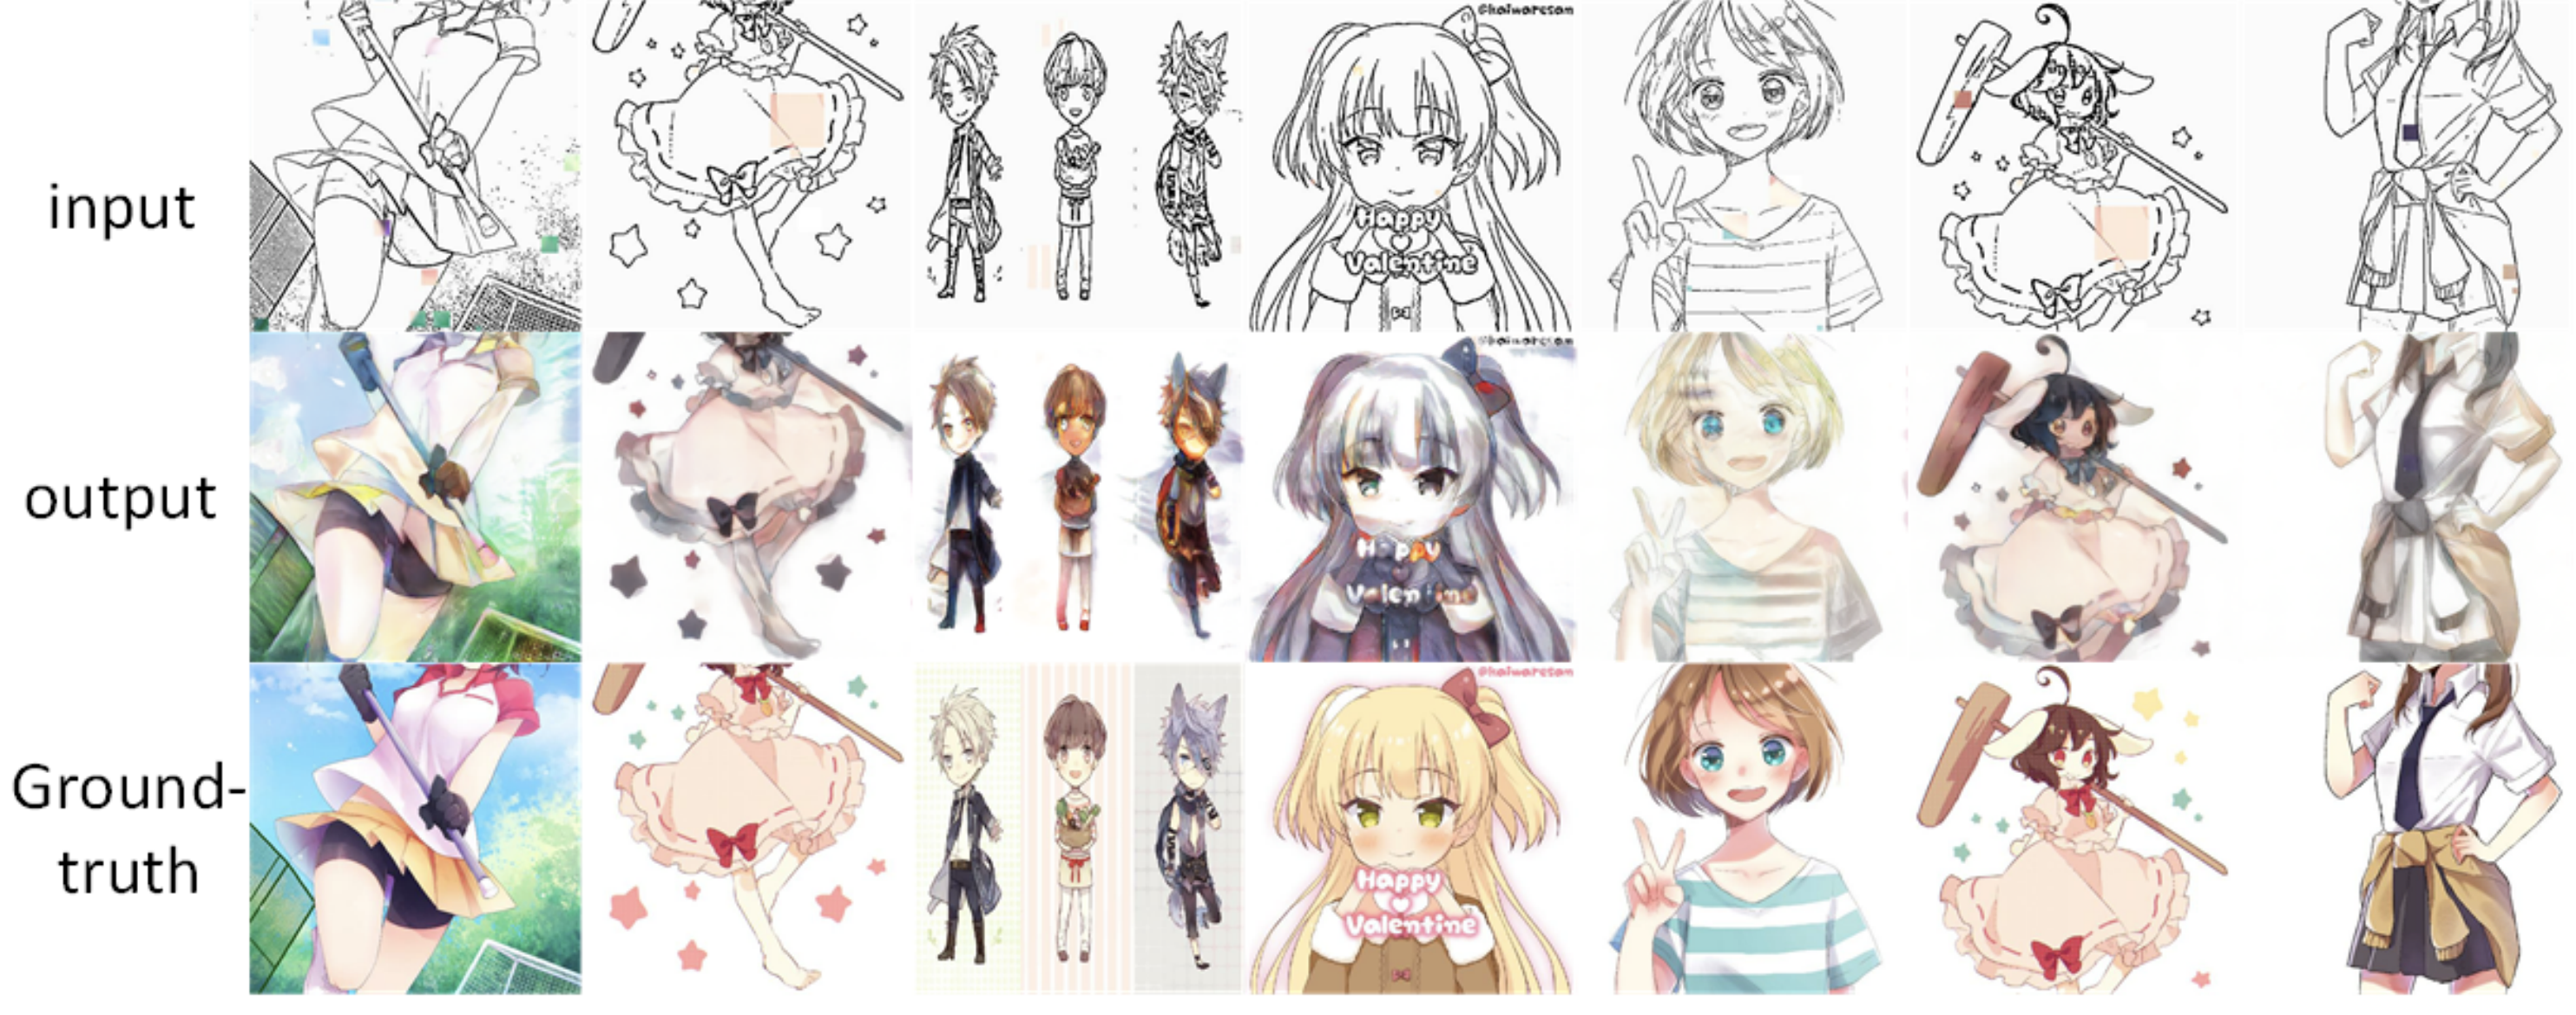
\includegraphics[width=0.9\textwidth]{autopainter}
	\caption{AutoPainter결과 예시}
	\label{fig:autopainter}
\end{figure}